\documentclass[14pt]{extarticle}

% Language setting
% Replace `english' with e.g. `spanish' to change the document language
\usepackage[english]{babel}

% Set page size and margins
% Replace `letterpaper' with `a4paper' for UK/EU standard size
\usepackage[letterpaper,top=2cm,bottom=2cm,left=2cm,right=2cm,marginparwidth=1.75cm]{geometry}

% Useful packages
\usepackage[fleqn]{amsmath}
\usepackage{amssymb}
\usepackage{graphicx}
\usepackage[colorlinks=true, allcolors=blue]{hyperref}
\usepackage{enumitem}

\usepackage{xcolor, soul}
\sethlcolor{yellow}

\setlength{\parindent}{0cm}

\title{MAT168 HW2}
\author{Andrew Jowe}

\begin{document}
\maketitle

\section*{(1)}
% ?? REDO with auxilery problem
\subsection*{Original Problem}
\[
    \zeta = 2x_1 - 6x_2 + 0x_3
\]
\[
    x_4 = -2 + x_1 + x_2 + x_3
\]
\[
    x_5 = 1 - 2x_1 + x_2 - x_3
\]

\subsection*{Setup}
\[
    N=\begin{bmatrix}
        -1 & -1 & -1 \\
        2 & -1 & 1 \\
    \end{bmatrix}
\]

\[
    B=\begin{bmatrix}
        1 & 0 \\
        0 & 1 \\
    \end{bmatrix}
\]

\[
    A
    =\left[NB\right]
    =\begin{bmatrix}
        -1 & -1 & -1 & 1 & 0 \\
        2 & -1 & 1 & 0 & 1 \\
    \end{bmatrix}
\]

\[
    b=\begin{bmatrix}
        -2 \\
        1 \\
    \end{bmatrix}
\]

\[
    c=\begin{bmatrix}
        2 \\
        -6 \\
        0 \\
        0 \\
        0 \\
    \end{bmatrix}
\]

\[
    x^*_B = \begin{bmatrix}
        x^*_4 \\
        x^*_5 \\
    \end{bmatrix}
    = \begin{bmatrix}
        -2 \\
        1 \\
    \end{bmatrix}
\]

\subsection*{Iteration 1}
\subsubsection*{Step 1}
\[
    x^*_B \ngeq 0
\]

\subsubsection*{Step 2}
\[
    z^*_N=-c_N=\begin{bmatrix}
        2 \\
        -6 \\
        0 \\
    \end{bmatrix}
\]

\[
    j = 2
\]

\subsubsection*{Step 3}
\[
    \Delta x_B = B^{-1}Ne_j
\]

\[
    \Delta x_B
    =\begin{bmatrix}
        1 & 0 \\
        0 & 1 \\
    \end{bmatrix}^{-1}
    \begin{bmatrix}
        -1 & -1 & -1 \\
        2 & -1 & 1 \\
    \end{bmatrix}
    \begin{bmatrix}
        0 \\
        1 \\
        0 \\
    \end{bmatrix}
\]

\[
    \Delta x_B = 
    \begin{bmatrix}
        -1 \\
        -1 \\
    \end{bmatrix}
\]

\subsubsection*{Step 4}
\[
    t = \left(max_{i \in B} \frac{\Delta x_i}{x^*_i}\right)^{-1}
\]

\[
    t = \left(max_{i \in B} \left\{ \frac{-2}{-1} _{\textstyle,}\ \frac{-1}{1} \right\} \right)^{-1}
\]

\[
    t = \frac{-1}{1}_{\textstyle,}
\]

\subsubsection*{Step 5}
\[
    i = 5
\]

\subsubsection*{Step 6}
\[
    \Delta z_N = -\left(B^{-1}N\right)^T e_i
\]

\[
    \Delta z_N = -\left(
    \begin{bmatrix}
        1 & 0 \\
        0 & 1 \\
    \end{bmatrix}^{-1}
    \begin{bmatrix}
        -1 & -1 & -1 \\
        2 & -1 & 1 \\
    \end{bmatrix}\right)^T
    \begin{bmatrix}
        0 \\
        1 \\
    \end{bmatrix}
\]

\[
    \Delta z_N =
    -\begin{bmatrix}
        -1 & -1 & -1 \\
        2 & -1 & 1 \\
    \end{bmatrix}^T
    \begin{bmatrix}
        0 \\
        1 \\
    \end{bmatrix}
\]

\[
    \Delta z_N =
    \begin{bmatrix}
        1 & -2 \\
        1 & 1 \\
        1 & -1 \\
    \end{bmatrix}
    \begin{bmatrix}
        0 \\
        1 \\
    \end{bmatrix}
\]

\[
    \Delta z_N =
    \begin{bmatrix}
        -2 \\
        1 \\
        -1 \\
    \end{bmatrix}
\]

\subsubsection*{Step 7}
\[
    s = \frac{z^*_j}{\Delta z_j} = \frac{-6}{1} = -6
\]

\subsubsection*{Step 8}
\[
    x^*_2 = 
\]

\section*{(2)}
% ??

\section*{(3)}
% ??
\subsubsection*{Optimal Dictionary}
\[
    \zeta = 13-3x_2-x_4-x_6
\]
\[
    x_3 = 1+x_2+3x_4-2x_6
\]
\[
    x_1 = 2-2x_2-2x_4+x_6
\]
\[
    x_5 = 1+5x_2+2x_4
\]

\subsubsection*{Given}
\[
    B = \{3, 1, 5\},\ N = \{2, 4, 6\}
\]
\[
    c = [5, 4, 3, 0, 0, 0]
\]
\[
    z^*_N = \begin{bmatrix}
        3 \\
        1 \\
        1 \\
    \end{bmatrix}
\]

\subsubsection*{Calculations}
\[
    -B^{-1}N = \begin{bmatrix}
        1 & 3 & -2 \\
        -2 & -2 & 1 \\
        5 & 2 & 0 \\
    \end{bmatrix}
\]

\subsubsection*{Range for $c_2$}
\[
    \Delta c = [0, 1, 0, 0, 0, 0]
\]
\[
    \Delta c^T_B = [0, 0, 0]
\]
\[
    \Delta c^T_N = [0, 1, 0]
\]

\bigskip Then:
\[
    \Delta z_N = (B^{-1}N)^T \Delta c_B - \Delta c_N
\]
\[
    \Delta z_N = \begin{bmatrix}
        1 & 3 & -2 \\
        -2 & -2 & 1 \\
        5 & 2 & 0 \\
    \end{bmatrix}^T
    \begin{bmatrix}
        0 \\
        0 \\
        0 \\
    \end{bmatrix}
    - \begin{bmatrix}
        0 \\
        1 \\
        0 \\
    \end{bmatrix}
\]

\bigskip Since $z^*_N + t\Delta z_N \geq 0$:
\[
    \begin{bmatrix}
        3 \\
        1 \\
        1 \\
    \end{bmatrix}
    + t \begin{bmatrix}
        % ??
        0
    \end{bmatrix}
    \geq \begin{bmatrix}
        0 \\
        0 \\
        0 \\
    \end{bmatrix}
\]

\subsubsection*{Range for $c_3$}
\[
    \Delta c = [0, 0, 1, 0, 0, 0]
\]

\section*{(4)}
\subsection*{Constraints}
The production facilities can produce 11k units per month. Let $\{x\}_1^3$ be the packages shipped from San Francisco and $\{x\}_4^6$ be the packages shipped from Sacramento.
\newline $x_1 + x_2 + x_3 \leq 11$
\newline $x_4 + x_5 + x_6 \leq 11$

\bigskip

We have to meet the demand at the destinations which is 10k at Davis, 8k at Winters, and 4k at Woodland. Let $x_1, x_4$ be the packages shipped to Davis. Let $x_2, x_5$ be the packages shipped to Winters. Let $x_3, x_6$ be the packages shipped to Woodland.
\newline $x_1 + x_4 \geq 10$
\newline $x_2 + x_5 \geq 8$
\newline $x_3 + x_6 \geq 4$

\subsection*{Objective Function}
We want to minimize cost of both facilities. Let vector $c$ be the cost to ship.
\newline $min\ c^Tx$
\newline $min\ 10x_1 + 8x_2 + 12x_3 + 4x_4 + 11x_5 + 6x_6$

\subsection*{Online Solver}
We used this online solver: https://online-optimizer.appspot.com

\subsubsection*{Input}
         var x1 $>=$ 0;
\newline var x2 $>=$ 0;
\newline var x3 $>=$ 0;
\newline var x4 $>=$ 0;
\newline var x5 $>=$ 0;
\newline var x6 $>=$ 0;

\bigskip minimize z: 10*x1 + 8*x2 + 12*x3 + 4*x4 + 11*x5 + 6*x6;

\bigskip subject to c11: x1 + x2 + x3 $<=$ 11;
\newline subject to c12: x4 + x5 + x6 $<=$ 11;
\newline subject to c13: x1 + x4 $>=$ 10;
\newline subject to c14: x2 + x5 $>=$ 8;
\newline subject to c15: x3 + x6 $>=$ 4;

\bigskip end;

\subsubsection*{Output Model Overview}
\begin{tabular}{|l|l|}
    \hline
    Label & Value \\
    \hline
    Problem type & Linear optimization \\
    \hline
    Objective & Minimize z \\
    \hline
    Optimal objective value & 146 \\
    \hline
    Solver Status & Optimal \\
    \hline
    Total number of variables & 6 \\
    \hline
    Continuous variables & 6 \\
    \hline
    Number of constraints & 6 \\
    \hline
    Non-binary nonzero coefficients & 18 \\
    \hline
\end{tabular}

\subsubsection*{Output Model Variables}
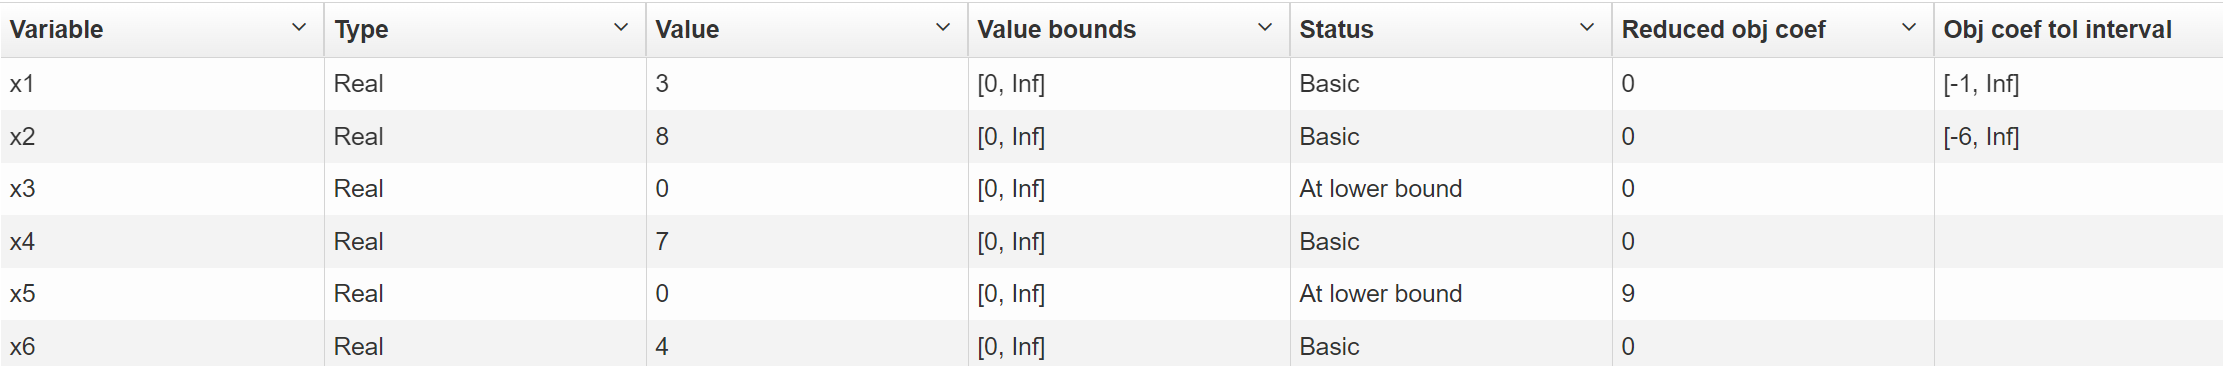
\includegraphics[width=\textwidth]{OutputVariables.PNG}

\subsubsection*{Output Model Constraints}
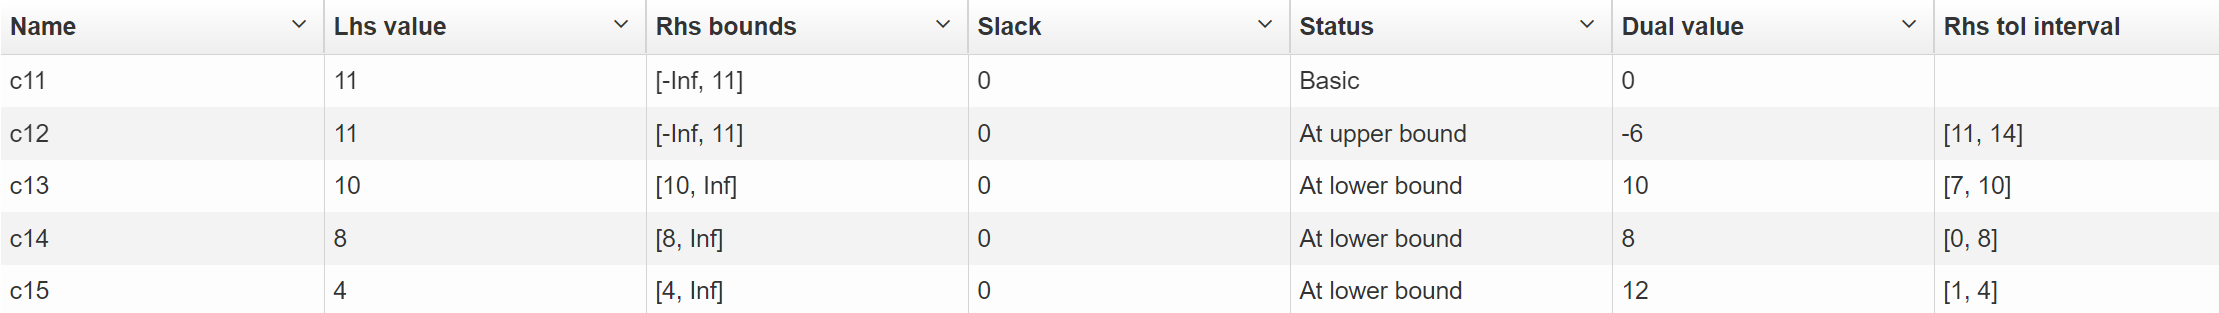
\includegraphics[width=\textwidth]{OutputConstraints.PNG}

\subsubsection*{Output Model Log Messages}
Reading model section from editor.mod ...
\newline 16 lines were read
\newline Generating z...
\newline Generating c11...
\newline Generating c12...
\newline Generating c13...
\newline Generating c14...
\newline Generating c15...
\newline Model has been successfully generated
\newline Scaling...
\newline  A: min|aij| = 1  max|aij| = 12  ratio = 12
\newline GM: min|aij| = 0.7681450856702011  max|aij| = 1.3018373985007101  ratio = 1.6947806121350972
\newline EQ: min|aij| = 0.6030226891555273  max|aij| = 1  ratio = 1.6583123951777
\newline Solving the model using the simplex optimizer
\newline GLPK Simplex Optimizer, v4.49
\newline 6 rows, 6 columns, 18 non-zeros
\newline Preprocessing...
\newline 5 rows, 6 columns, 12 non-zeros
\newline Scaling...
\newline  A: min|aij| = 1  max|aij| = 1  ratio = 1
\newline Problem data seem to be well scaled
\newline Constructing initial basis...
\newline Size of triangular part = 5
\newline  0: obj = 0  infeas = 22 (0)
\newline *4: obj = 209  infeas = 0 (0)
\newline *6: obj = 146  infeas = 0 (0)
\newline OPTIMAL SOLUTION FOUND

\section*{Collaboration}
All collaborators are listed (in alphabetical order) below:
\begin{itemize}
    \item Anne
    \item Jack
    \item Dhruv
    \item Fengqin
    \item Zhongning
    \item Sterling
\end{itemize}

\section*{Academic Integrity}
On my personal integrity as a student and member of the UCD community, I have not given, nor received and unauthorized assistance on this assignment.

Signature: Andrew Jowe

\end{document}